\documentclass[preprint2]{aastex}

\usepackage{url}
\usepackage{multirow}
\usepackage{amsmath}
\usepackage{xcolor}
\usepackage{mathrsfs}
%\citestyle{aa}

%\bibliographystyle{apj_w_etal}

\newcommand{\etal}{{et al.\/}}
\newcommand{\Prob}{\mathtt{P}}
\newcommand{\logL}{\log\mathcal{L}}
\newcommand{\unit}[1]{\footnotesize #1}
\newcommand{\PAPER}{\mathrm{PAPER}}
\newcommand{\hMpci}{h\ {\rm Mpc}^{-1}}

\newcommand{\Nx}{$N_x$}
\newcommand{\MminX}{$M_{minX}$}
\newcommand{\alphaX}{$\alpha_X$}
\newcommand{\xray}{X-ray}

\newcommand{\HI}{HI}
%%define graphics path to search for images
%\graphicspath{{./data/}}

%\usepackage[justification=centering]{caption}

\definecolor{orange}{RGB}{255,127,0}

\tabletypesize{\scriptsize}

	% End definitions

%\slugcomment{DRAFT: \today}

\shorttitle{ECHO}
\shortauthors{Jacobs et al.}

\begin{document}


\title{The External Calibrator for Hydrogen Arrays}
\author{
Daniel C. Jacobs\altaffilmark{1},
Jacob Burba\altaffilmark{1},
Judd Bowman\altaffilmark{1},
Lauren Turner\altaffilmark{1},
Kali Johnson\altaffilmark{1}}
\altaffiltext{1}{School of Earth and Space Exploration, Arizona State U., Tempe, AZ, 85287}



\begin{abstract}
We describe the External Calibrator for Hydrogen Observatories (ECHO) 
\end{abstract}



\section{Introduction}\label{sec:intro}

\section{Design and Method}

The ECHO system utilizes a X8 octoquad drone manufactured by 3DRobotics (3DR) with an onboard, programmable Valon 5007 synthesizer and a BicoLOG 30100 biconical antenna.  Capable of broadcasting between 137.5-4400 MHz, the Valon synth can be programmed to 

\section{Calibration}
\subsection{Maps}
\subsection{Comparison to Orbcomm ratio maps}
\section{MWA Tile}
\subsection{data}
\subsection{systematic variation}
\subsection{comparison to orbcomm maps}
\section{Conclusion}


\section{Acknowledgments}{

ECHO is supported by a grant from the National Science Foundation (NSF; award number 1407646). D.C.J would like to acknowledge NSF support  under award 1401708.
Thanks to the National Radio Astronomy Observatory, Green Bank and to Embry Riddle Aeronautical Observatory for cooperatively supporting site operations.
}
\bibliographystyle{apj}
\bibliography{library}


% Figures at end?

\onecolumn
\begin{center}

\begin{figure}[h]
\centering
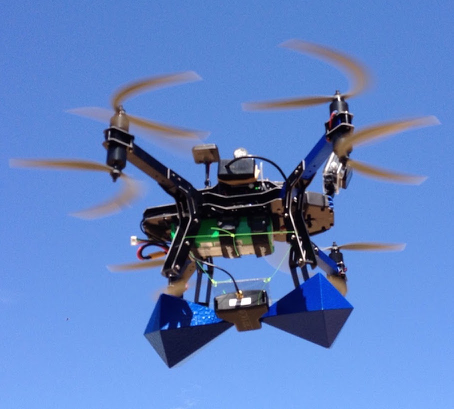
\includegraphics[scale=0.5]{images/drone.png}
\caption{Drone in flight}
\label{fig:Drone}
\end{figure}

\begin{figure}[h]
\centering
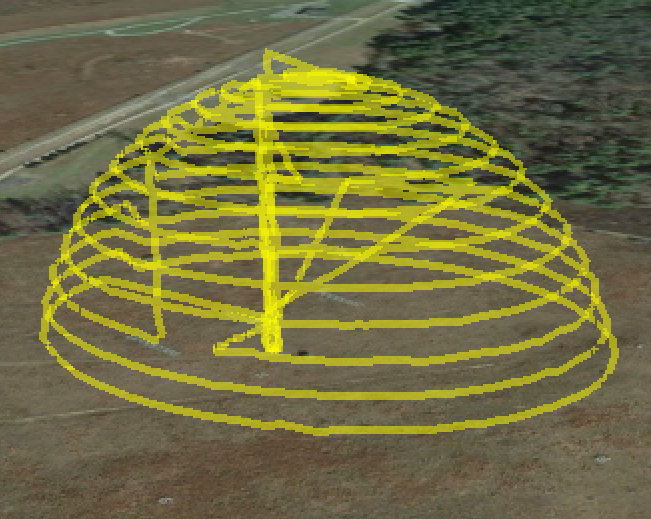
\includegraphics[scale=0.7]{images/flight_path.png}
\caption{Flight path of drone in Green Bank, WV}
\label{fig:Flight path}
\end{figure}

\begin{figure}[h]
\centering
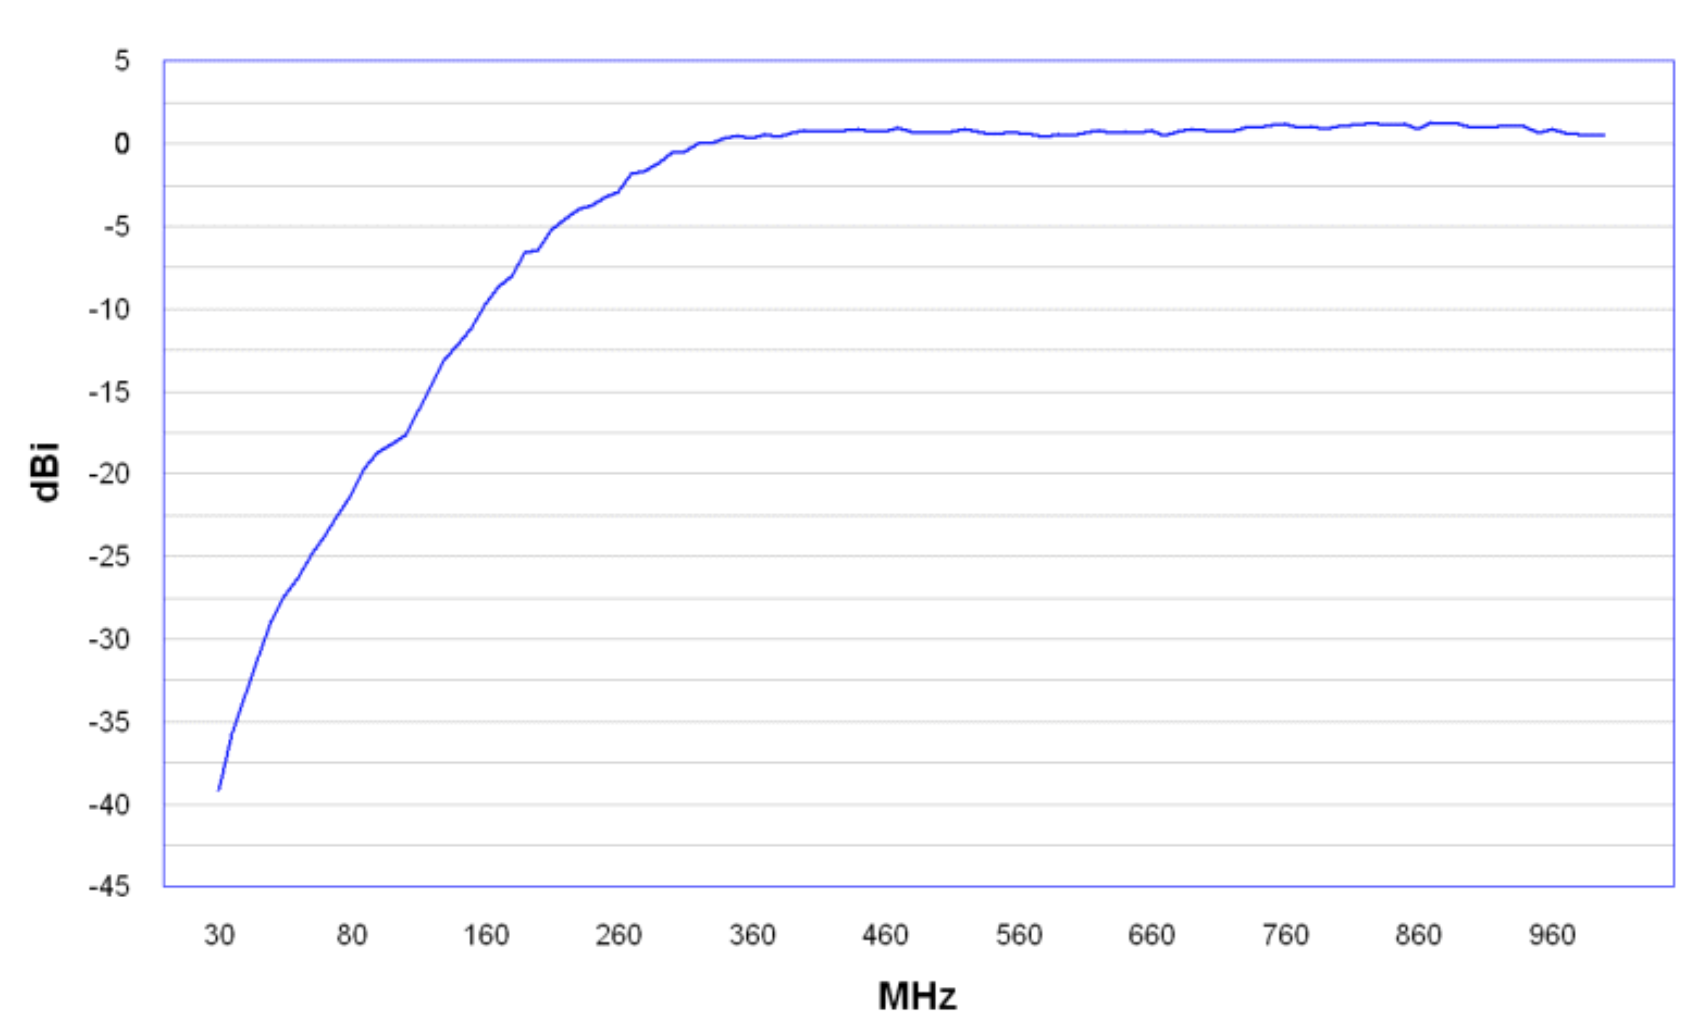
\includegraphics[scale=0.5]{images/bicolog_frequency_response.png}
\caption{Frequency response of BicoLOG 30100 biconical antenna.}
\label{BicoLOG response}
\end{figure}

\begin{figure}[h]
\centering
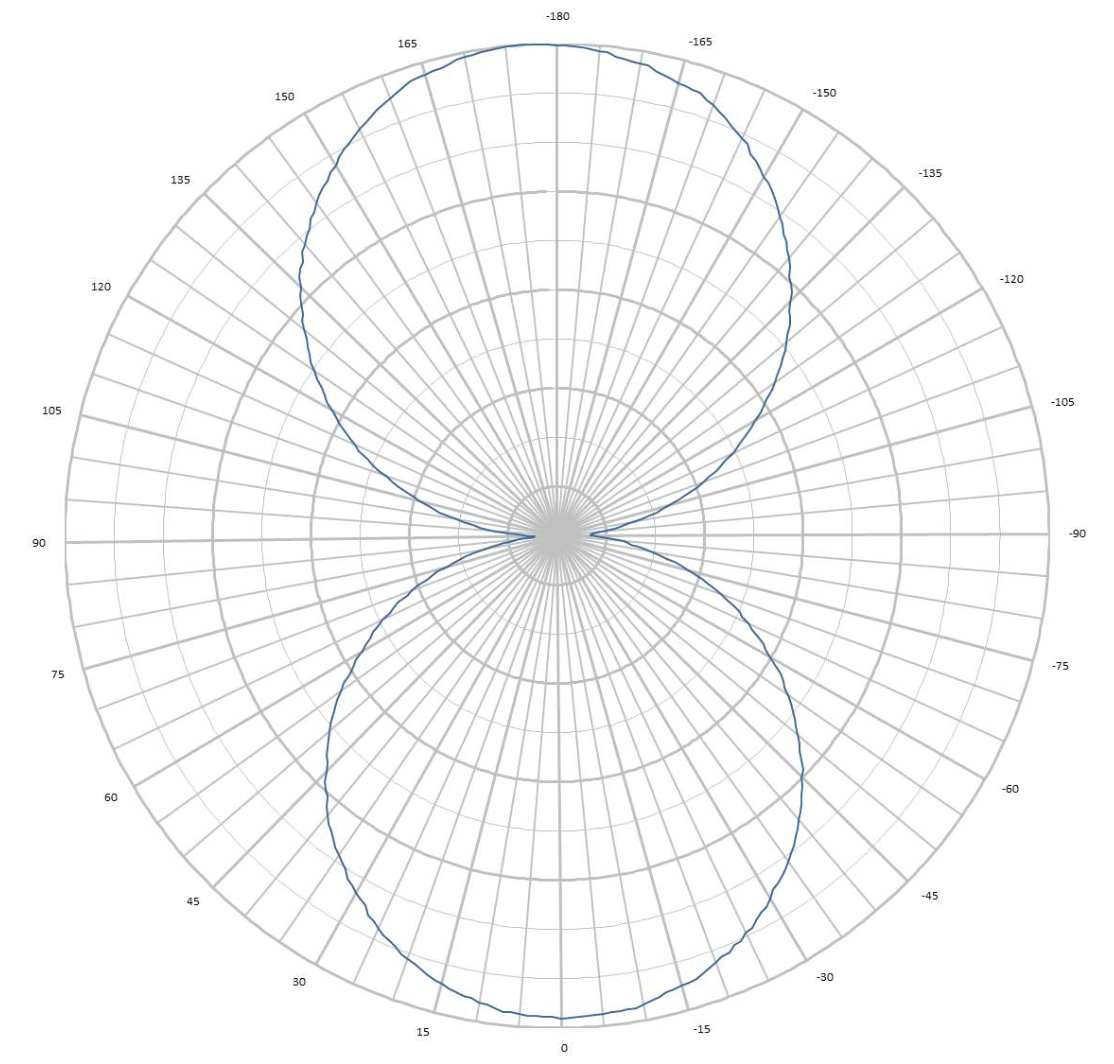
\includegraphics[scale=0.4]{images/bicolog_horizontal_cut.png}
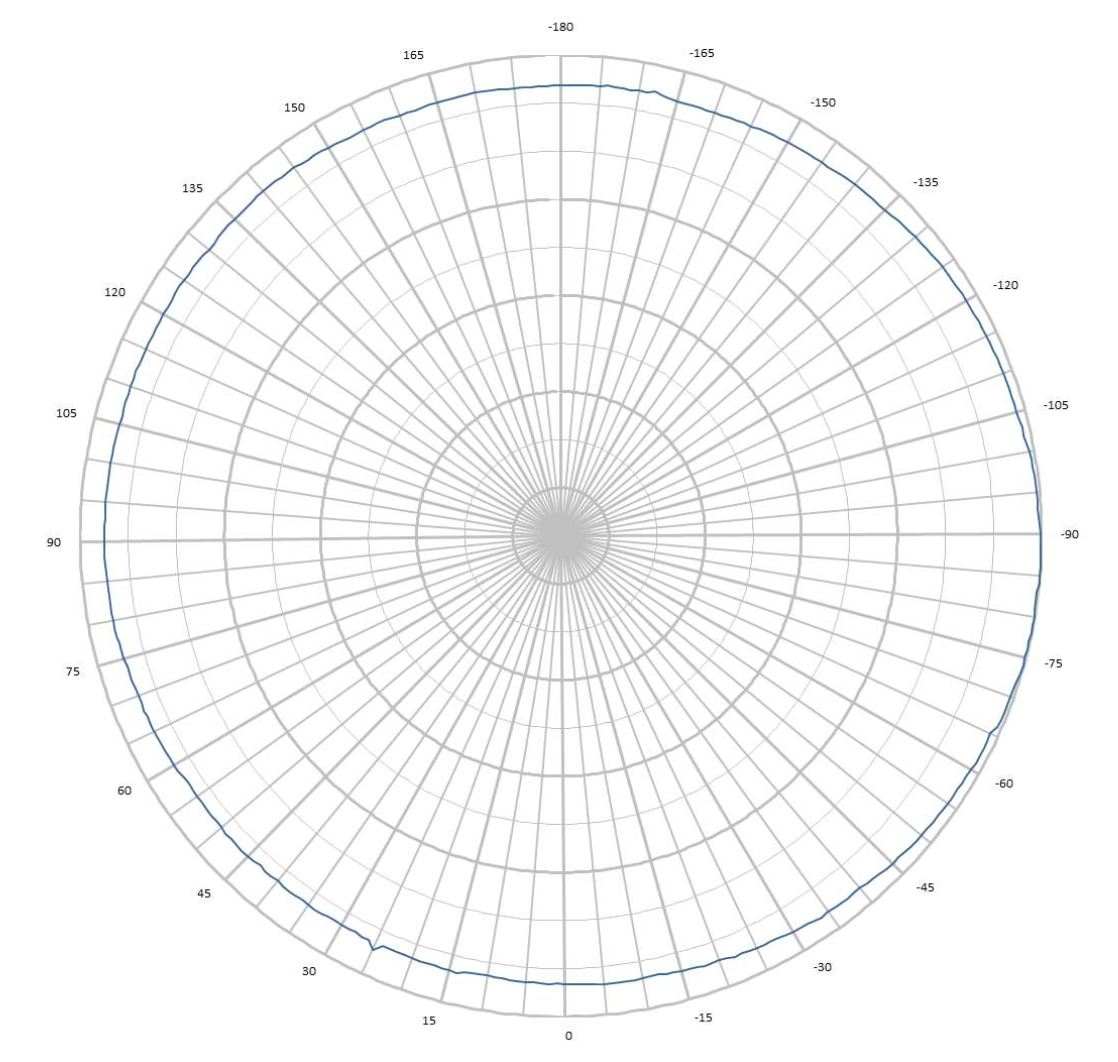
\includegraphics[scale=0.4]{images/bicolog_vertical_cut.png}
\caption{Horizontal (left) and vertical (right) cut through BicoLOG beam.}
\label{fig:BicoLOG cuts}
\end{figure}

\end{center}

\end{document}
